\chapter{Cross-country comparison: Italy and Sweden}
\label{ch:ch5}

This chapter extends the segmentation framework of Chapter~\ref{ch:ch4} to Sweden, applying identical preprocessing and clustering rules on the Swedish sub-sample, and then compares the two country segmentations at the profile level. The comparison is motivated by the polar welfare-regime contrast --- Italy's familistic model against Sweden's universalist model (Esping-Andersen, 1990; Ferrera, 1996) --- and the expectation that the same analytical pipeline should yield profile structures that rhyme across countries while differing systematically in levels.

\section{The six Swedish profiles}
\label{sec:ch5-swedish-profiles}

The Swedish analytical sample comprises $n = 1{,}787$ respondents, obtained from the $2{,}202$ first-implicate over-65 Swedes after complete-case listwise deletion ($n = 2{,}045$) and the removal of 258 Mahalanobis outliers at the $\chi^{2}$ cut-off of $p = 0.001$ with 31 degrees of freedom. Unlike Italy, Sweden retains all thirty-one analytical variables in the clustering input: \emph{ac035d4} and \emph{ac035d7} exhibit low but non-zero variance (four to six per cent positive responses) and therefore contribute to the analysis.

K-means with $k = 6$ on the standardised-variable matrix yields six interpretable profiles (Table~\ref{tab:ch5-swedish-profiles}). The solution is retained at $k = 6$ without the micro-cluster removal step applied to Italy, since no micro-cluster smaller than five per cent of the sample emerges from the Swedish fit.

\begin{table}[ht]
  \centering
  \caption{Swedish profile sizes and cluster means on key variables ($n = 1{,}787$).}
  \label{tab:ch5-swedish-profiles}
  \small
  \begin{tabular}{@{}lrrrrrrrr@{}}
    \toprule
    \textbf{Profile} & \textbf{n} & \textbf{\%} & \textbf{Age} & \textbf{Internet} & \textbf{CASP} & \textbf{Lone.} & \textbf{Hope} & \textbf{LifeSat}\\
    \midrule
    Fragile            & 206 & 11.5 & 80.4 & 0.64 & 33.6 & 4.9 & 0.81 & 7.42\\
    Social Decline     & 149 &  8.3 & 72.6 & 0.99 & 40.3 & 3.5 & 0.98 & 8.51\\
    Moderate           & 417 & 23.3 & 76.6 & 0.94 & 37.1 & 3.8 & 0.91 & 8.06\\
    Asset Rich         & 341 & 19.1 & 77.7 & 0.75 & 39.3 & 3.8 & 0.96 & 8.48\\
    Wealthy Digital    & 138 &  7.7 & 74.9 & 0.96 & 40.3 & 3.5 & 0.99 & 8.47\\
    Connected Wealthy  & 536 & 30.0 & 73.1 & 0.99 & 42.1 & 3.3 & 0.99 & 8.88\\
    \bottomrule
  \end{tabular}
  \par\smallskip
  \footnotesize \emph{Note.} Internet and Hope are binary proportions. Profile ordering within the table is alphabetical; the substantive ordering in the text follows CASP ascending from Fragile to Connected Wealthy.
\end{table}

Two features distinguish the Swedish segmentation from the Italian one. First, three out of six Swedish profiles have internet penetration above 94\% --- a level that in Italy is approached only by Connected Active. Second, even the most fragile Swedish profile (Fragile, CASP = 33.6) reports subjective well-being comparable to the Italian Fragile Depressed (CASP = 30.7) or Moderate Isolated (CASP = 36.8) profiles, confirming a structural welfare-regime gap that is visible across the entire distribution rather than concentrated at the margins.

\subsection{Fragile}
The smallest and oldest profile ($n = 206$; 11.5\%; mean age 80.4) is the Swedish counterpart of the Italian Fragile Resigned: low CASP (33.6), high loneliness (4.9), reduced hope (81\%). Internet use is 64\%, dramatically higher than the Italian Fragile Resigned (9\%) at comparable age and clinical conditions.
\subsection{Social Decline}
A compact profile ($n = 149$; 8.3\%) characterised by intact digital integration (99\% internet) but elevated loneliness (3.5) and a CASP of 40.3. It is the Swedish analogue of the Italian Fragile Depressed.
\subsection{Moderate}
The largest middle-aged profile ($n = 417$; 23.3\%) combines good health, average digital use (94\%), and moderate social integration (loneliness 3.8, CASP 37.1). It maps onto the Italian Traditional Social in the matched-pair framework introduced below.
\subsection{Asset Rich}
A wealth-driven profile ($n = 341$; 19.1\%) with high life satisfaction (8.48) but below-average internet use (75\%) and smaller social networks than Connected Wealthy. It has no Italian analogue and is one of the two welfare-regime-specific Swedish types.
\subsection{Wealthy Digital}
The smallest Swedish profile ($n = 138$; 7.7\%) combines very high internet use (96\%), high CASP (40.3), and strong hope (99\%). Like Asset Rich, this is a Swedish-specific type with no Italian counterpart.
\subsection{Connected Wealthy}
The largest Swedish profile ($n = 536$; 30.0\%) represents the upper tail of the distribution: near-universal internet use (99\%), lowest loneliness (3.3), highest CASP (42.1), highest life satisfaction (8.88). It is the Swedish counterpart of the Italian Connected Active.

\section{Matched-pair comparison}
\label{sec:ch5-matched-pairs}

The cross-country comparison uses the four matched pairs introduced in Table~\ref{tab:ch3-matched-pairs}. Table~\ref{tab:ch5-gap} reports the Sweden-minus-Italy gap on seven outcome variables for each of the four pairs.

\begin{table}[ht]
  \centering
  \caption{Cross-country gap (Sweden minus Italy) on matched profile pairs.}
  \label{tab:ch5-gap}
  \small
  \begin{tabular}{@{}lrrrr@{}}
    \toprule
    \textbf{Variable} & \textbf{Fragile} & \textbf{Declining} & \textbf{Socially-oriented} & \textbf{Connected}\\
    \midrule
    CASP-12             & $+5.73$   & $+9.63$   & $-1.37$   & $+4.31$\\
    Loneliness (3--9)   & $-1.24$   & $-1.90$   & $+0.07$   & $-0.45$\\
    Internet (pp)       & $+55.0$   & $+81.4$   & $+28.0$   & $+23.7$\\
    Fluency             & $+8.67$   & $+13.61$  & $+4.18$   & $+7.30$\\
    Hope (pp)           & $+35.2$   & $+30.4$   & $+1.21$   & $+8.55$\\
    EURO-D (0--12)      & $-2.29$   & $-2.23$   & $+1.21$   & $-0.80$\\
    Life satisfaction   & $+0.97$   & $+1.34$   & $-0.13$   & $+0.76$\\
    \bottomrule
  \end{tabular}
  \par\smallskip
  \footnotesize \emph{Note.} Matched pairs: \emph{Fragile} = Fragile Resigned vs Fragile; \emph{Declining} = Fragile Depressed vs Social Decline; \emph{Socially-oriented} = Traditional Social vs Moderate; \emph{Connected} = Connected Active vs Connected Wealthy. Internet and Hope are expressed in percentage points (of the binary rate). Loneliness and EURO-D negative values mean Sweden is lower (less lonely, less depressed) than Italy.
\end{table}

Welch's $t$-tests on every cell of Table~\ref{tab:ch5-gap} confirm that all gaps in the Fragile, Declining and Connected pairs are statistically significant at $p < 0.01$, with most of them at $p < 10^{-15}$. The Socially-oriented pair is the only exception: on loneliness, Hope, and life satisfaction, Traditional Social Italians and Moderate Swedes are indistinguishable; on CASP, the Italian Traditional Social exceeds the Swedish Moderate by $1.37$ points ($p = 0.001$), the only case in which Italy \emph{leads} Sweden in the matched-pair design. Figure~\ref{fig:ch5-matched-pairs-gap} visualises the same comparison.

\begin{figure}[ht]
  \centering
  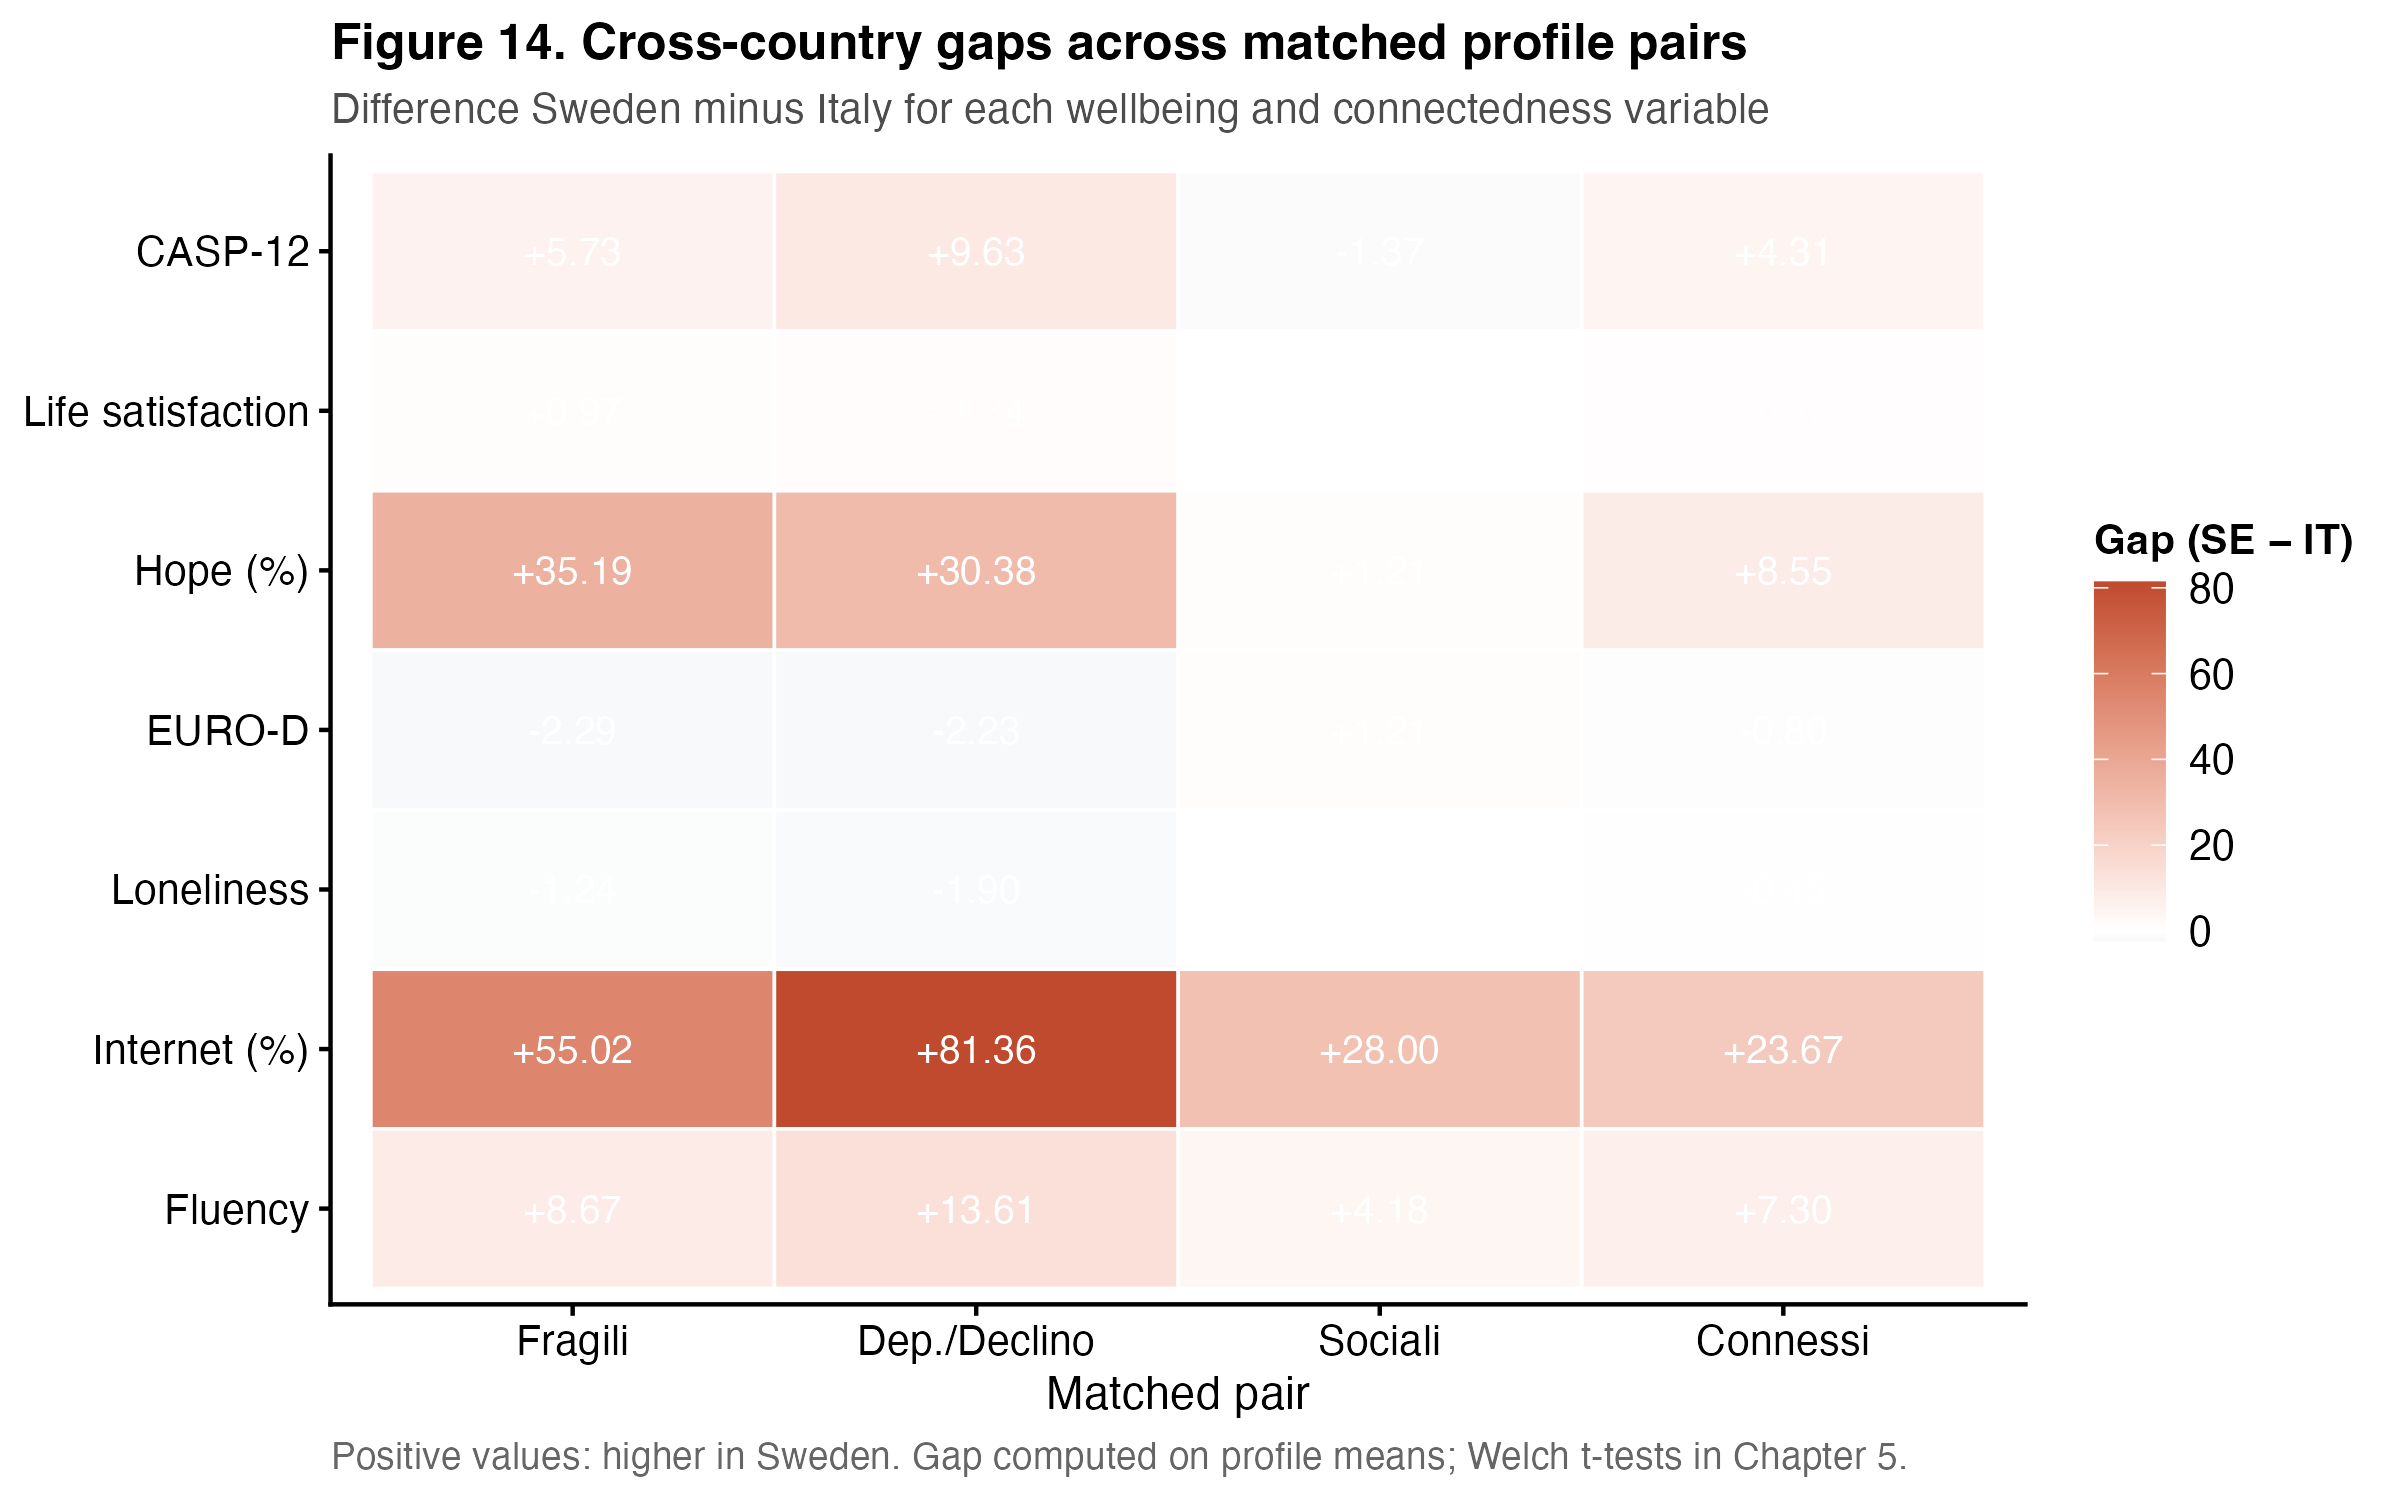
\includegraphics[width=0.90\linewidth]{figures/06_comparison/fig_14_matched_pairs_gap.png}
  \caption{Sweden-minus-Italy gap by matched pair, seven outcome variables. Source: v9 pipeline.}
  \label{fig:ch5-matched-pairs-gap}
\end{figure}

\section{The systematic Swedish-over-Italian gap}
\label{sec:ch5-gap}

The quantitative pattern of Table~\ref{tab:ch5-gap} can be summarised as follows. On CASP-12, Swedes exceed matched Italians by between $+4.31$ (Connected pair) and $+9.63$ (Declining pair), with the largest gap falling on the most vulnerable groups. On the internet variable, the gap ranges from $+23.7$ percentage points (Connected pair) to $+81.4$ points (Declining pair) --- essentially a wholesale transformation of the digital-access profile at the bottom of the distribution. On fluency, Swedes outperform Italians by 4 to 14 words per minute, with the same distribution-concentration pattern. On depression (EURO-D), Swedes score between $0.80$ and $2.29$ points lower, with the gap again largest among the most fragile.

The gap is therefore \emph{structural} rather than compositional: the same analytical pipeline applied to both samples reveals a Sweden-over-Italy shift that is preserved across profiles, rules out sample-level composition effects, and is largest at the vulnerable end of each distribution. The interpretation in terms of welfare-regime architecture is developed in Chapter~\ref{ch:ch8}.

\section{Welfare-regime-specific profiles}
\label{sec:ch5-unmatched}

Three profiles fall outside the matched-pair design and are interpreted as welfare-regime-specific types. The Italian \emph{Moderate Isolated} ($n = 639$) is the large objectively-healthy-but-socially-isolated group that is absent from the Swedish segmentation; its substantive importance is developed in Chapter~\ref{ch:ch7}. On the Swedish side, \emph{Asset Rich} ($n = 341$) and \emph{Wealthy Digital} ($n = 138$) are two prosperous profiles that occupy different positions in the digital-access space (75\% vs 96\% internet use, respectively) and in the social-network dimension; together they account for 26.8\% of the Swedish sample and have no Italian analogue. Figure~\ref{fig:ch5-country-unique} displays the unique profiles in each country.

\begin{figure}[ht]
  \centering
  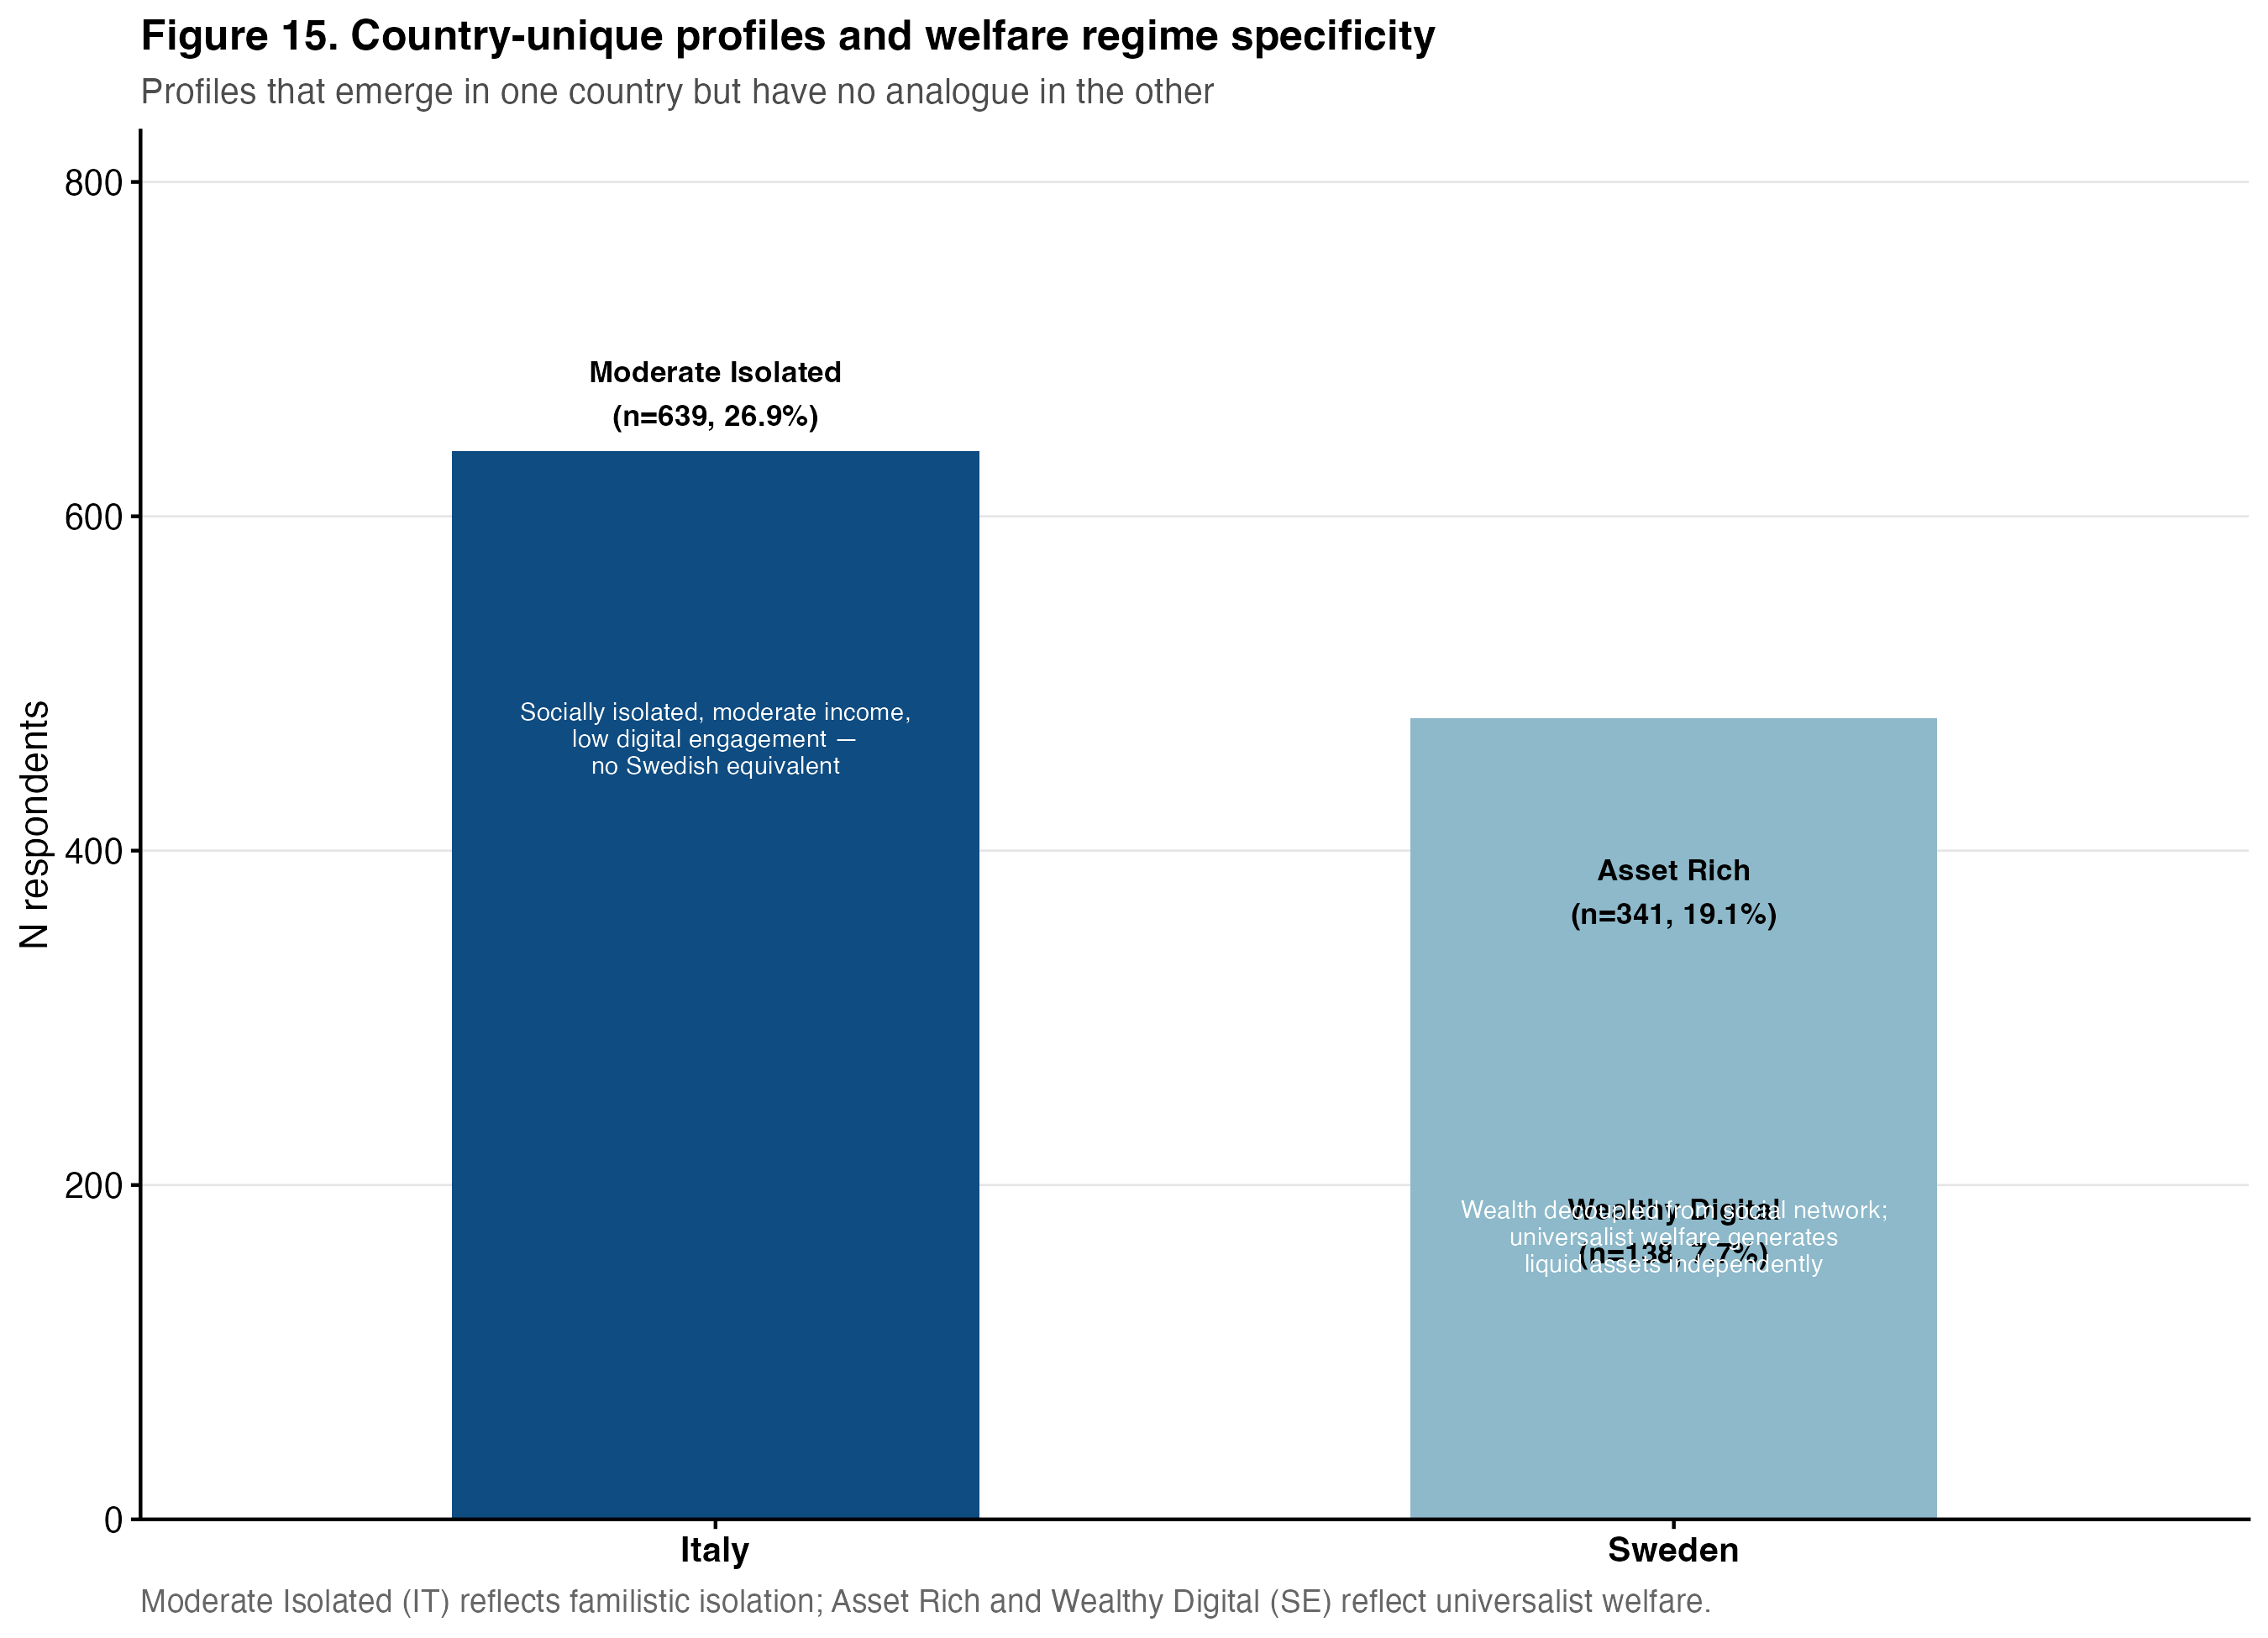
\includegraphics[width=0.78\linewidth]{figures/06_comparison/fig_15_country_unique.png}
  \caption{Welfare-regime-specific profiles in Italy and Sweden. Source: v9 pipeline.}
  \label{fig:ch5-country-unique}
\end{figure}

\section{Pooled latent space}
\label{sec:ch5-pooled}

As an additional check on cross-country commensurability, PCA and factor analysis were re-estimated on the pooled $n = 4{,}165$ sample after joint standardisation. Figure~\ref{fig:ch5-pc-pooled} and Figure~\ref{fig:ch5-fa-pooled} show respondents from both countries in the first principal-component and principal-axis planes respectively. The two country distributions overlap substantially on the second axis but separate on the first --- consistent with a shared latent structure and a country-specific level gradient, i.e.\ the same interpretation supported by Table~\ref{tab:ch5-gap}.

\begin{figure}[ht]
  \centering
  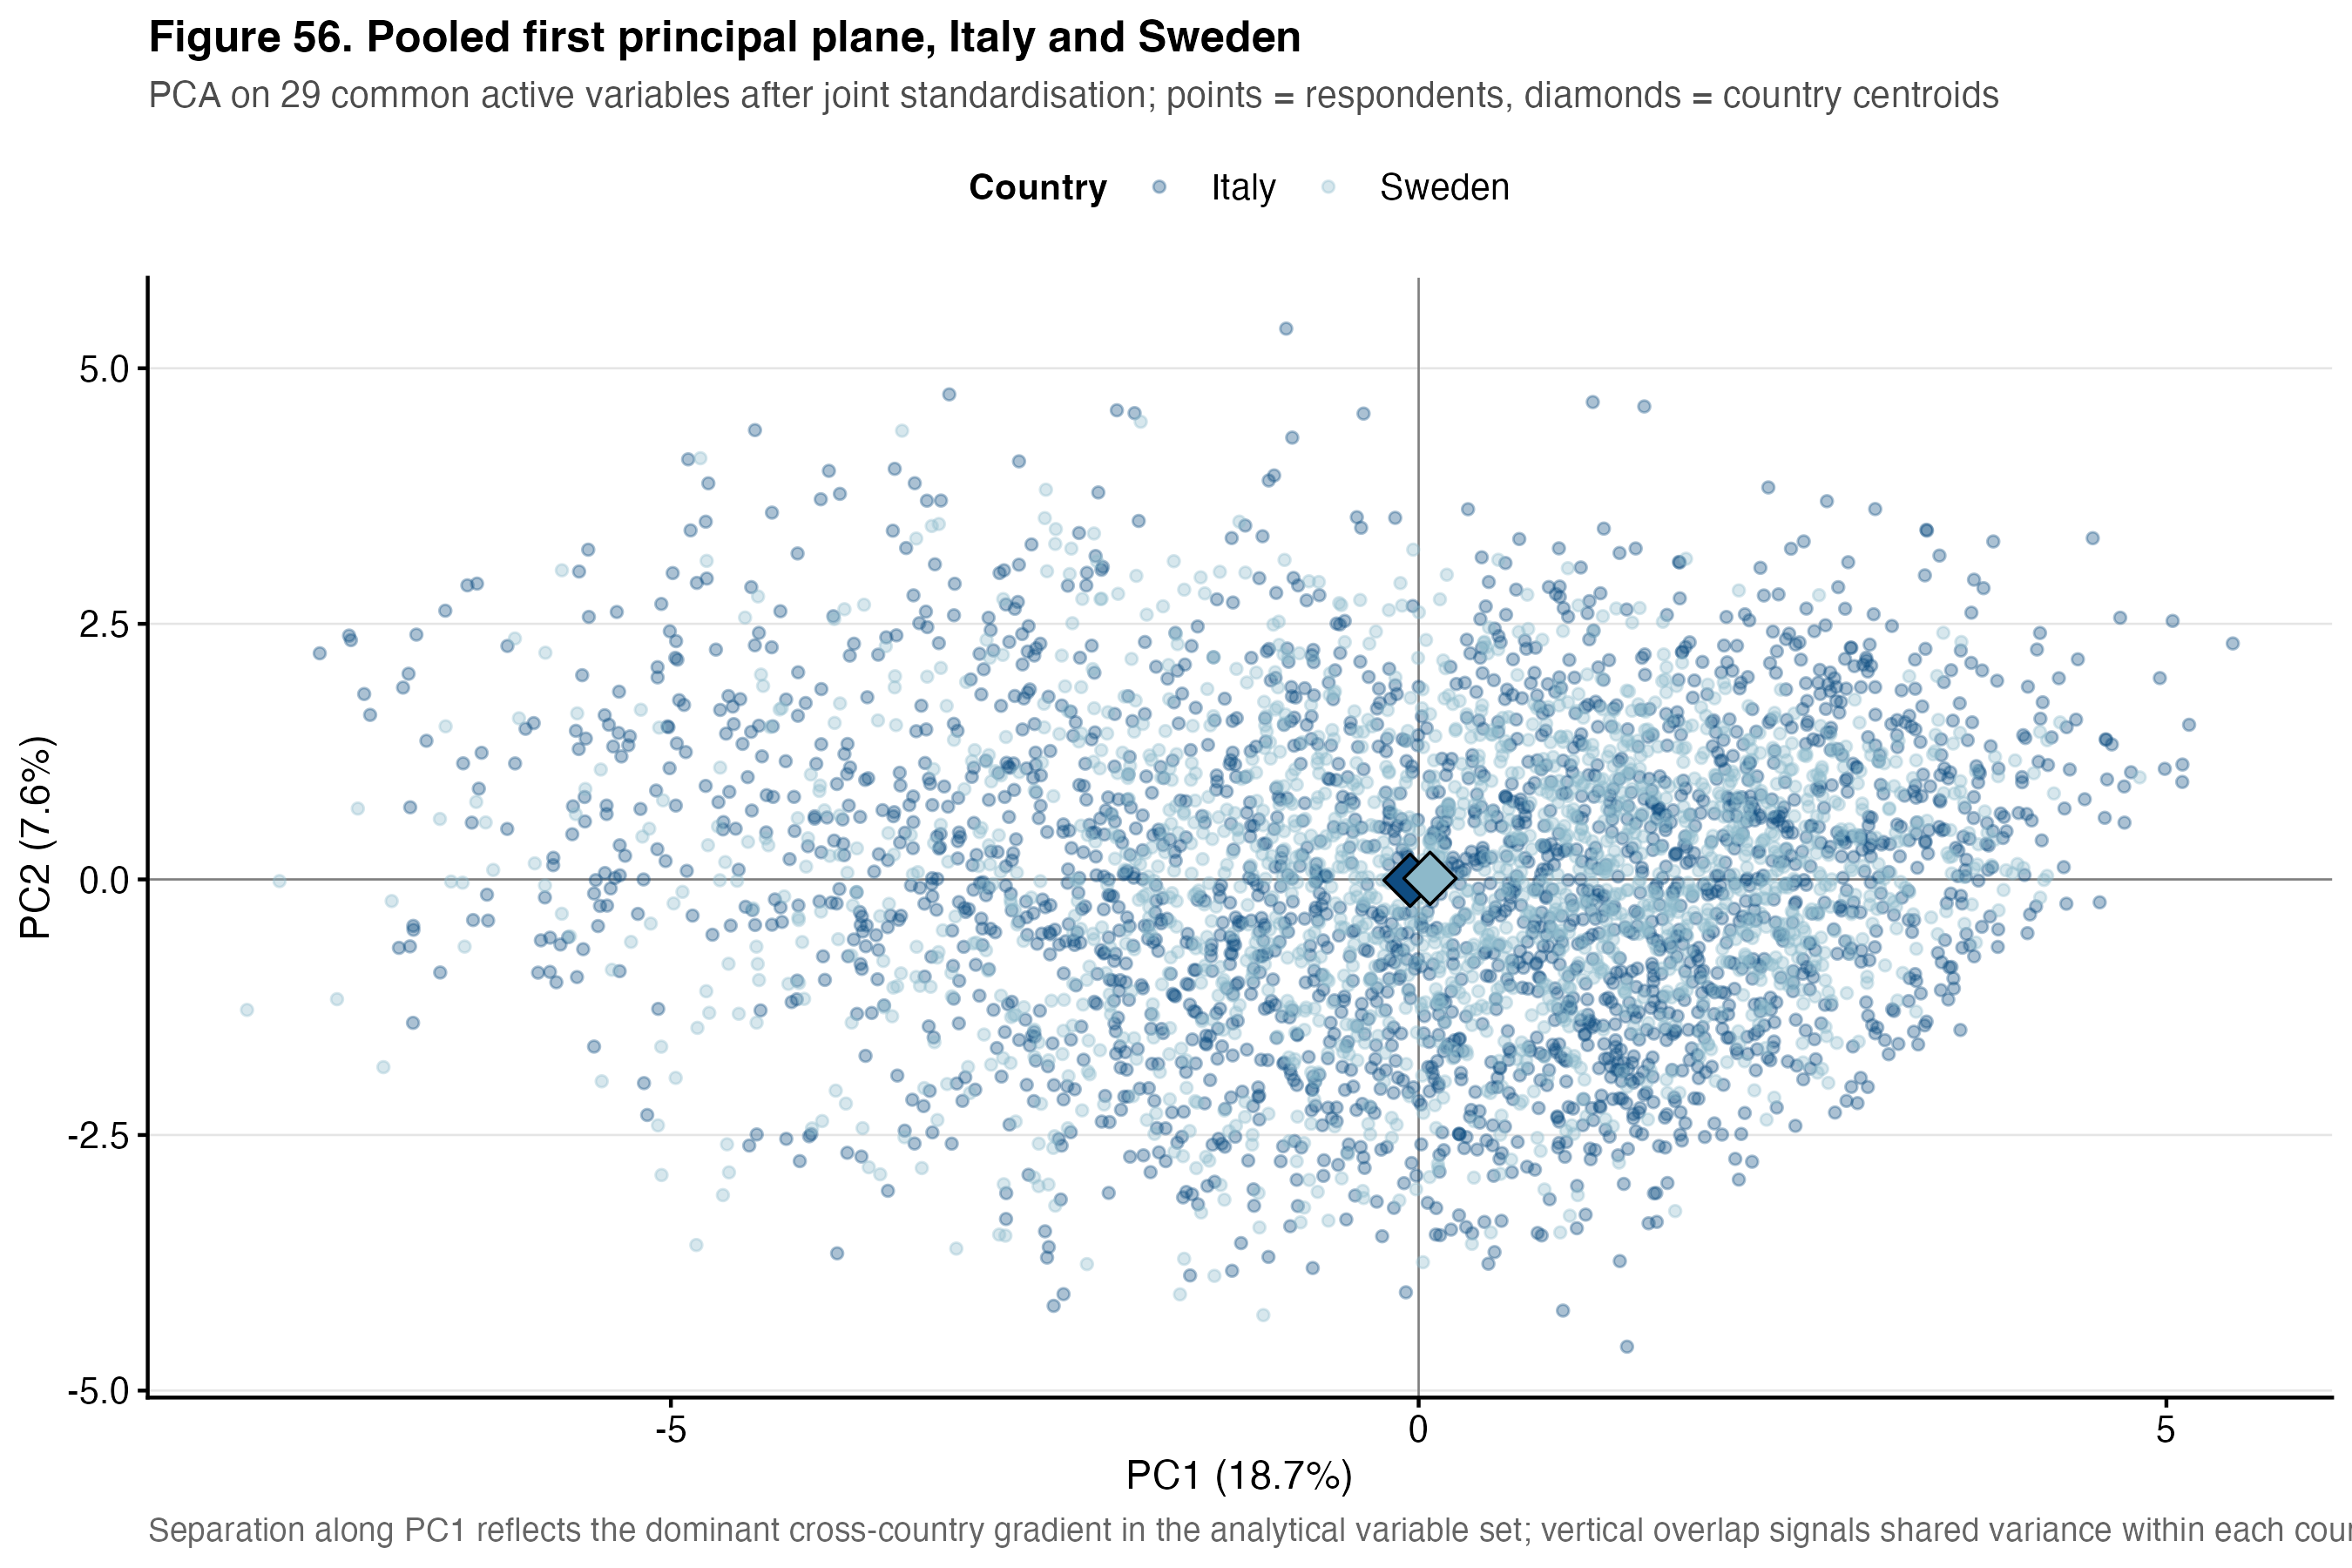
\includegraphics[width=0.85\linewidth]{figures/06_comparison/fig_56_pc_pooled_by_country.png}
  \caption{Respondents in the pooled PC1--PC2 space, coloured by country. Source: v9 pipeline.}
  \label{fig:ch5-pc-pooled}
\end{figure}

\begin{figure}[ht]
  \centering
  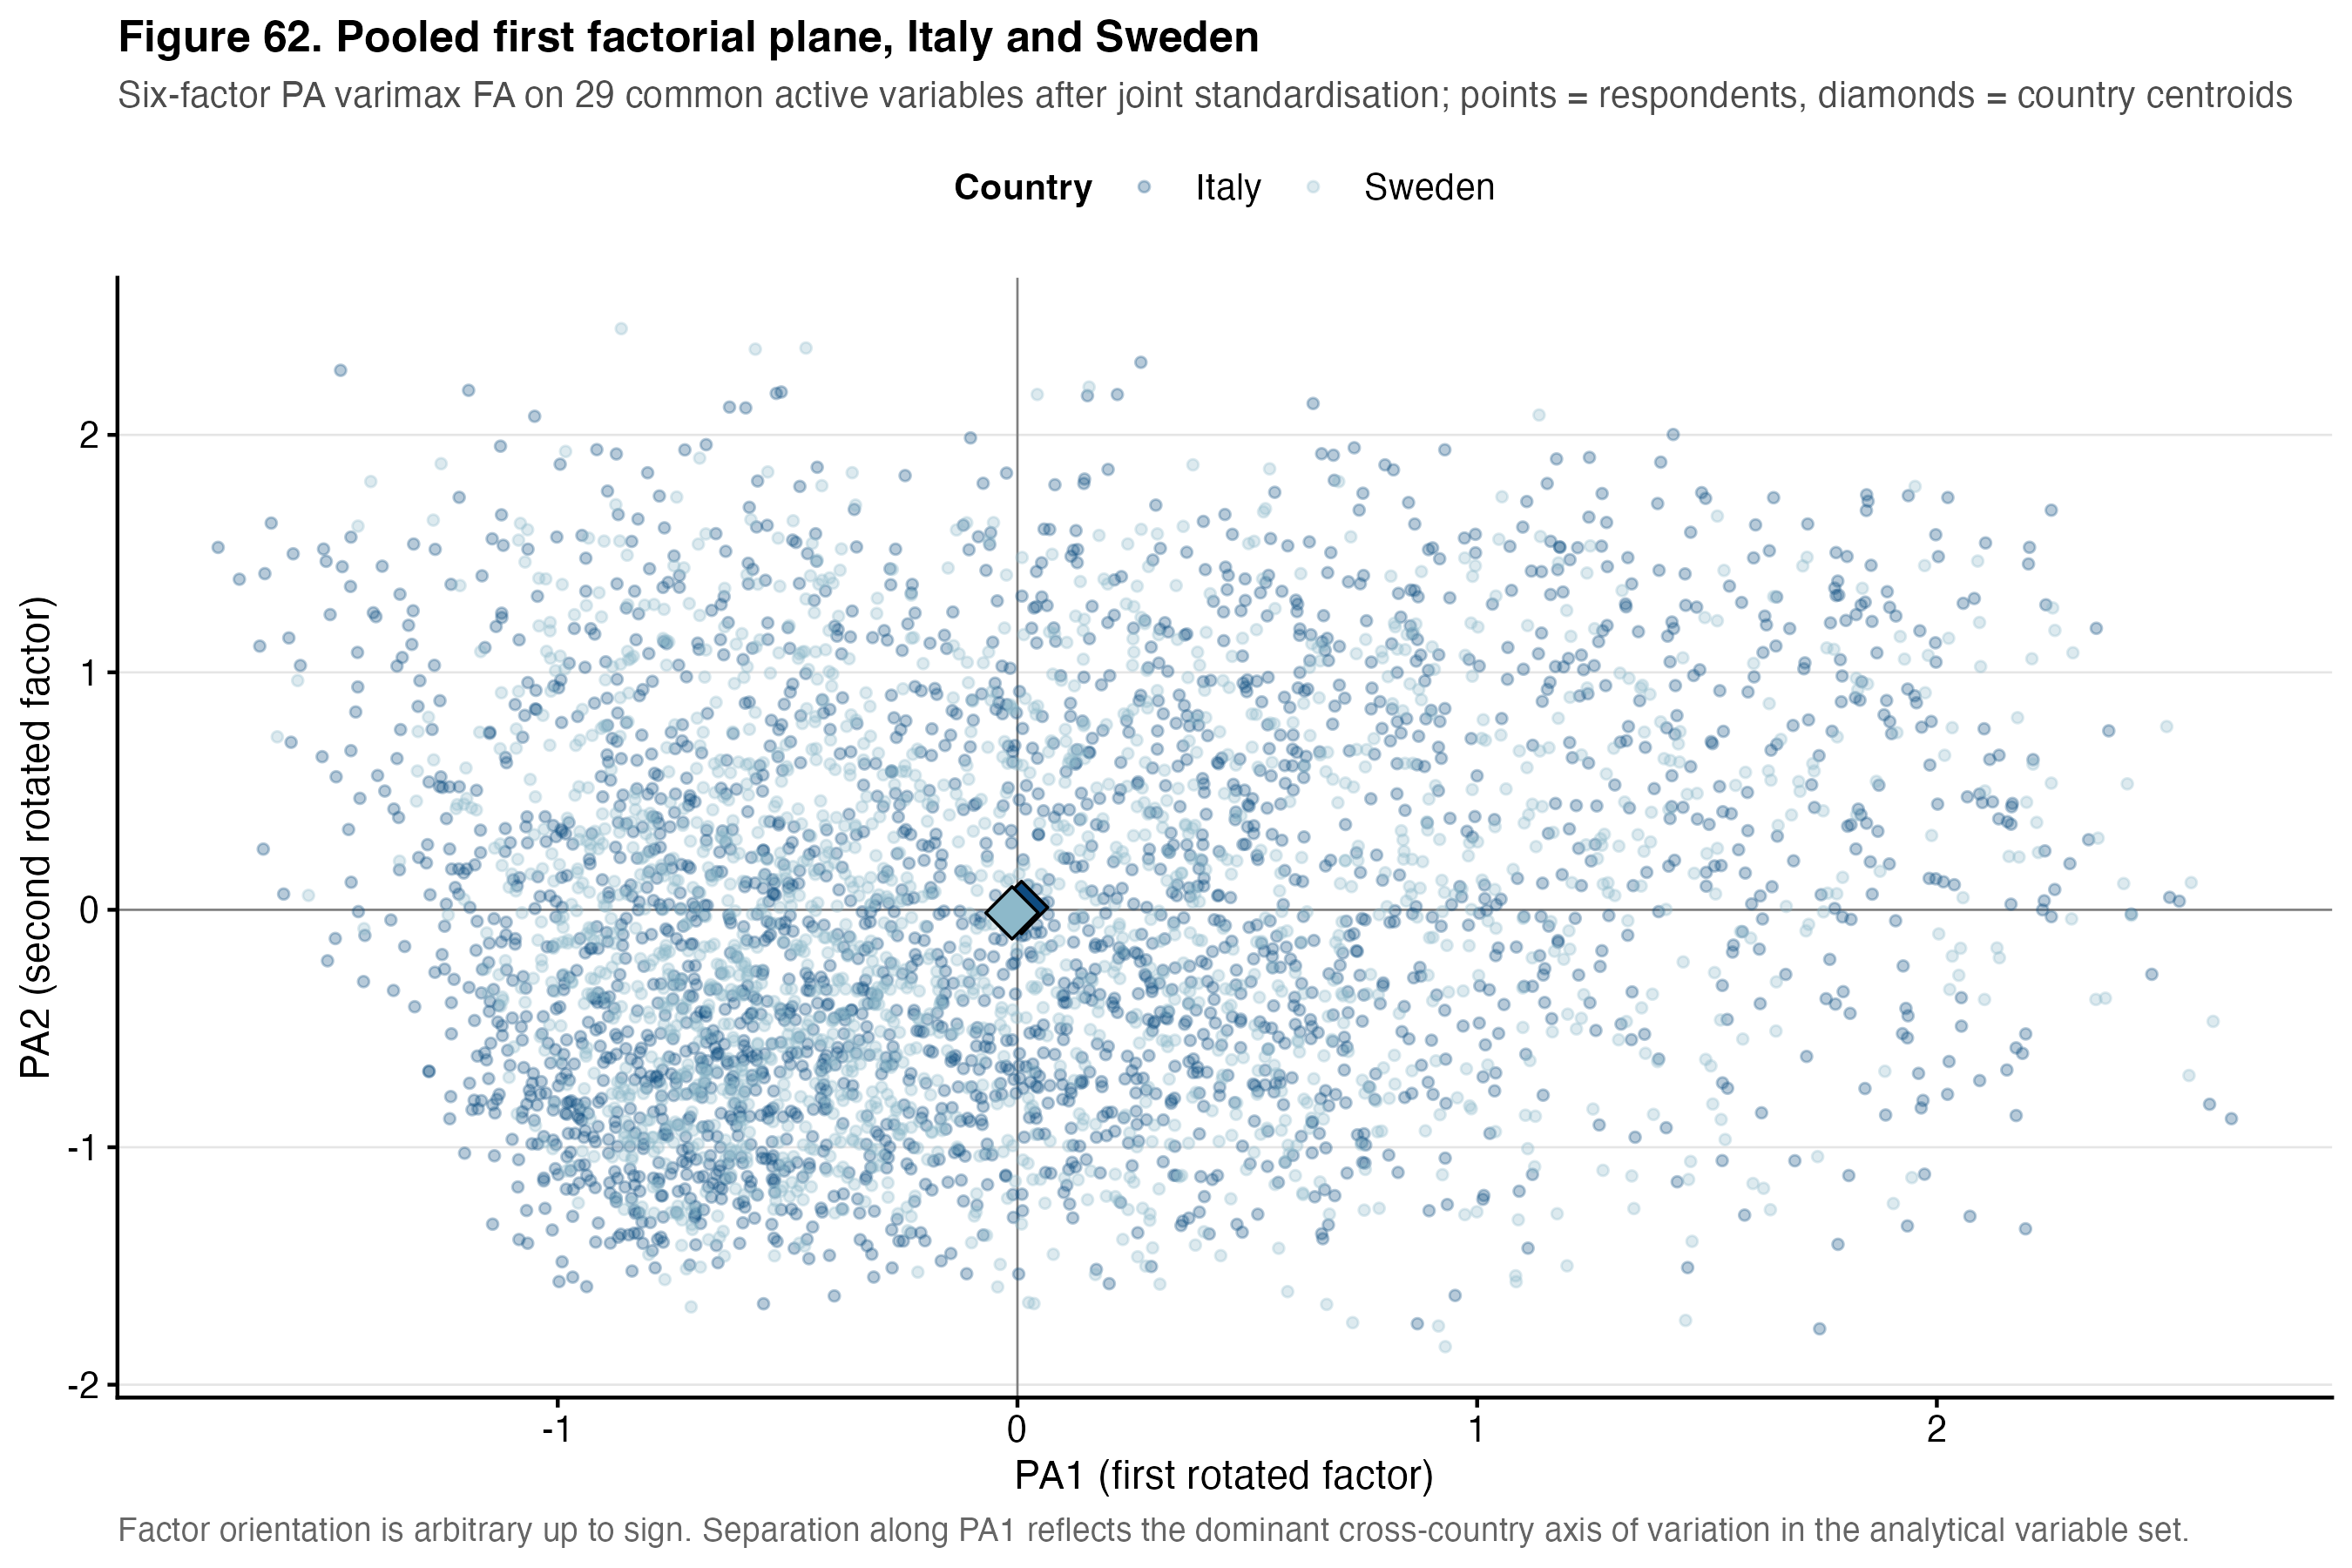
\includegraphics[width=0.85\linewidth]{figures/06_comparison/fig_62_fa_pooled_by_country.png}
  \caption{Respondents in the pooled PA1--PA2 factor-score space, coloured by country. Source: v9 pipeline.}
  \label{fig:ch5-fa-pooled}
\end{figure}

\section{Chapter summary}
\label{sec:ch5-summary}

The same analytical pipeline produces rhyming profile structures in Italy and Sweden, confirming the cross-country usability of the segmentation framework. Within this common structure, Sweden exceeds Italy on every positive indicator of subjective well-being, cognitive function, and digital inclusion, with gaps that are largest for the most vulnerable profiles. Two profiles have no cross-country analogue: the Italian \emph{Moderate Isolated}, whose characterisation prepares the healthcare chapter that follows, and the Swedish \emph{Asset Rich} and \emph{Wealthy Digital} types, interpretable as welfare-regime-specific signatures of the universalist model.
